\documentclass[usenames,dvipsnames]{beamer}
    \mode<presentation> {
    \usetheme{Montpellier}
    \usecolortheme{beaver}
    %\setbeamertemplate{footline} % To remove the footer line in all slides uncomment this line
    \setbeamertemplate{footline}[page number] % To replace the footer line in all slides with a simple slide count uncomment this line
    \setbeamertemplate{navigation symbols}{} % To remove the navigation symbols from the bottom of all slides uncomment this line
    }

    \usepackage{graphicx} % Allows including images
    \usepackage{booktabs} % Allows the use of \toprule, \midrule and \bottomrule in tables
    \usepackage[outputdir=target]{minted}
    \usepackage{xcolor}
    \usepackage[utf8]{inputenc}
    \usepackage{pifont}
    \usepackage{xspace}
    \usepackage{newunicodechar}
    \newunicodechar{✪}{\ding{74}}

    \definecolor{mintedbackground}{rgb}{0.95,0.95,0.95}
    \newcommand{\code}[1]{\colorbox{lightgray}{\texttt{#1}}}
    \newcommand{\distage}{\texttt{distage}\xspace}

\newminted{scala}{
    bgcolor=mintedbackground,
    fontfamily=tt,
    linenos=true,
    numberblanklines=true,
    numbersep=5pt,
    gobble=0,
    frame=leftline,
    framerule=0.4pt,
    framesep=2mm,
    funcnamehighlighting=true,
    tabsize=4,
    obeytabs=false,
    mathescape=false
    samepage=false, %with this setting you can force the list to appear on the same page
    showspaces=false,
    showtabs =false,
    texcl=false,
}

\newminted{text}{
    bgcolor=mintedbackground,
    fontfamily=tt,
    linenos=true,
    numberblanklines=true,
    numbersep=5pt,
    gobble=0,
    frame=leftline,
    framerule=0.4pt,
    framesep=2mm,
    funcnamehighlighting=true,
    tabsize=4,
    obeytabs=false,
    mathescape=false
    samepage=false, %with this setting you can force the list to appear on the same page
    showspaces=false,
    showtabs =false,
    texcl=false,
}

\newminted{json}{
    bgcolor=mintedbackground,
    fontfamily=tt,
    linenos=true,
    numberblanklines=true,
    numbersep=5pt,
    gobble=0,
    frame=leftline,
    framerule=0.4pt,
    framesep=2mm,
    funcnamehighlighting=true,
    tabsize=4,
    obeytabs=false,
    mathescape=false
    samepage=false, %with this setting you can force the list to appear on the same page
    showspaces=false,
    showtabs =false,
    texcl=false,
}

    \setminted{fontsize=\footnotesize,baselinestretch=1}

    \usepackage{tikz}
    \usetikzlibrary{positioning}
    \graphicspath{{target/media/}}

    \title[\distage]{\distage: Modern Staged Dependency Injection for Scala}

    \institute[Septimal Mind Ltd]
    {
    Septimal Mind Ltd\\
    \medskip
    \textit{team@7mind.io}
    }
    \date{\today}

\begin{document}

% \begin{VerbatimOut}{ex-scala-roles.tmp}
% @RoleId("testservice")
% class TestService[F[_] : Monad](http: HttpSrv[F])
%   extends IzService {
%     override def start(): Unit = http.start()
%     override def stop(): Unit = http.stop()
% }
% class TestPlugin extends PluginDef {
%   many[IzService].add[TestService[IO]]
% }
% object TestLauncher {
%   // run with
%   // java test.jar test-service other-service
%   def main(args: Array[String]): Unit = IzRoleApp(args).main()
% }
% \end{VerbatimOut}

\begin{frame}
%\titlepage
\begin{figure}
\Huge
\color{RubineRed} dist✪ge
\noindent
\rule{\linewidth}{1mm}
\Large Modern Staged Dependency Injection for Scala
\rule{\linewidth}{1mm}
\end{figure}

\begin{figure}
\color{RubineRed}
\normalsize Modular Functional Programming \\
with \\
Context Minimization \\
through \\
Garbage Collection
\end{figure}

\begin{figure}
\Large Septimal Mind Ltd \\
\medskip
\textit{team@7mind.io}
\end{figure}

\end{frame}

%%%%%%%%%%%%%%%%%%%%%%%%%%%%%%%%%%%%%%%%%%%%%%%%%%%%%%%%%%%%%%%%%%%%%%%%%%%%%%%%%%%%%%%%%%%%%%%%%%%
\section{The problem: Dependency Injection and Functional Programming}

\begin{frame}
\frametitle{DI is outdated and doesn't compose with FP?}
  Many Scala folks think that:
  \begin{enumerate}
  \item DI is heavy and slow
  \begin{itemize}
    \item \textit{``tests initialize longer than they execute''}
  \end{itemize}
  \item DI is unsafe
  \begin{itemize}
    \item \textit{``my program may compile but fail on startup after a huge delay''}
  \end{itemize}
  \item DI doesn't work for modern FP code
  \begin{itemize}
    \item \textit{``we cannot inject \code{IO\lbrack\_, \_\rbrack} into \code{Repository\lbrack\_\lbrack\_, \_\rbrack\rbrack}''}
  \end{itemize}
  \item DI is full of magic and error-prone
  \begin{itemize}
    \item \textit{``I've read 80\% out of 5000-page Spring manual but still don't understand why do I need to put these twelwe annotations here.
    Also I've tried Guice but it failed with 10-megabytes stack after five minutes and 300 retries of database connection instantiation''}
  \end{itemize}
  \end{enumerate}


\end{frame}

\begin{frame}[fragile]
\frametitle{TLDR}
  \begin{scalacode}
import distage._, scalaz.zio.IO

trait Repository[F[_, _]] {}
class ProductionRepository[F[_, _]]() extends Repository[F]
class DummyRepository[F[_, _]]() extends Repository[F]
class App[F[_, _]](repository: Repository[F]) { def run = ??? }

class MyAppProd[F[_, _]] extends PluginDef {
  make[Repository[F]].from[ProductionRepository[F]]
  make[App[F]]
}
class Main[F[_, _]] { def main(args: Array[String]): Unit = {
  Injector()
    .produce(MyAppProd[F], roots = Set(DIKey.get[App[F]]))
    .run { app: App[F] => app.run() }
}}
object Main[IO]
  \end{scalacode}
\end{frame}

%%%%%%%%%%%%%%%%%%%%%%%%%%%%%%%%%%%%%%%%%%%%%%%%%%%%%%%%%%%%%%%%%%%%%%%%%%%%%%%%%%%%%%%%%%%%%%%%%%%
\section{\distage{} features}
\begin{frame}
  \frametitle{\distage: overview}
  \begin{enumerate}
    \item Staged Model: \textit{plans the job first then do},
    \item Garbage Collection: \textit{instantiates reachable instances only},
    \item Higher-Kinded Types support: \textit{injects typeclass instances},
    \item Path-Dependent Types support,
    \item Plan introspection: \textit{dumps, graphviz, dependency trees},
    \item Plan rewriting,
    \item Roles: \textit{multiple services in one process},
    \item Dynamic Plugins\footnotemark[2] and Testkit,
    \item Circular Dependencies\footnotemark[1],
    \item Trait Augmentation and Assisted Injection\footnotemark[1],
    \item Automatic Sets: \textit{prepopulated sets all the instances of a class}
  \end{enumerate}
  \footnotetext[1]{Both run-time and compile-time support}
  \footnotetext[2]{Run-time with compile-time verification}
\end{frame}

\begin{frame}
\frametitle{Garbage Collection for better and faster tests}
  \begin{enumerate}
    \item Define all your test and production dependencies as a flat list,
    \item Put discrimination tags on test-specific definitions,
    \item Only the instances required for your tests will be instantiated,
    \item It takes just milliseconds, not like in Spring,
    \item $\Rightarrow$ Significant savings on test startup time.
    \item You don't need to setup your context, it's done automatically by Plugin Loader and Garbage Collector,
    \item $\Rightarrow$ Substantial savings on test context configuration.
  \end{enumerate}
\end{frame}

\begin{frame}[fragile]
\frametitle{Example: Garbage Collection and tests}
  \begin{scalacode}
import distage._, scalaz.zio.IO

trait Repository[F[_, _]] {}
class ProductionRepository[F[_, _]]() extends Repository[F]
class DummyRepository[F[_, _]]() extends Repository[F]

class MyAppDef[F[_, _]] extends PluginDef {
  make[Repository[F]].from[ProductionRepository[F]]
  make[Repository[F]].tagged("test").from[DummyRepository[F]]
}

object MyApp extends MyApp[IO]

class RepoTest extends DistagePluginSpec { "repository" must {
"do something" in di {
  (repository: Repository[IO]) => // repository is a GC root
    // ProductionRepository will not be instantiated!
} } }
  \end{scalacode}
\end{frame}

\begin{frame}[fragile]
\frametitle{Garbage Collection for deployment: flexible monoliths}
  We may fuse Microservices with Monoliths keeping \textit{all} their benefits:
  \begin{enumerate}
  \item Develop software components (\textit{Roles}\footnotemark[1]) as usual\footnotemark[2],
  \item Each Role is a Garbage Collection Root,
  \item Build one Docker image with multiple Roles in it,
  \item Define Roles you want to start as commandline parameters,
  \item $\Rightarrow$ higher computational density, savings on infrastructure,
  \item $\Rightarrow$ \textit{substantial} development simplification: full environment may be started on a low-end machine with one command,
  \end{enumerate}

  \begin{textcode}
server1# docker run company/product +analytics
server2# docker run company/product +accounting +users
developer1# docker run company/product +*
developer2# docker run company/product --dummy-repositories +*
  \end{textcode}

  \footnotetext[1]{Slides with more details: https://goo.gl/iaMt43}
  \footnotetext[2]{You are not prohibited from using multirepo layout}
\end{frame}

\begin{frame}[fragile]
\frametitle{Config support}
  \distage has \texttt{HOCON} configuration extension.

  \begin{scalacode}
case class HostPort(host: String, port: Int)

class HttpServer(@ConfPath("http.listen") listenOn: HostPort) {
  // ...
}
  \end{scalacode}

  The extension:
  \begin{enumerate}
  \item Enumerates all the missing references in a Plan,
  \item Searches them for a specific \mintinline{scala}{@ConfPath} annotation,
  \item Tries to find corresponding sections in config source,
  \item Extends plan with config values,
  \item $\Rightarrow$ Config values are being resolved before instantiation begins,
  \item $\Rightarrow$ problems are being shown quickly and all at once.
  \end{enumerate}
\end{frame}

\begin{frame}[fragile]
  \frametitle{Dynamic Plugins}
  Just drop your modules into your classpath:
  \begin{scalacode}
class AccountingModule extends PluginDef {
  make[AccountingService].from[AccountingServiceImpl]
  // ...
}
  \end{scalacode}
  Then you may pick up all the modules and build your context:
  \begin{scalacode}
val plugins = new PluginLoaderDefaultImpl(
  PluginConfig(Seq("com.company.plugins"))
).load()
// ... pass to an Injector
  \end{scalacode}
  \begin{enumerate}
  \item Useful while you are prototyping your app,
  \item In maintenance phase you may switch to static configuration.
  \end{enumerate}
\end{frame}

\begin{frame}
  \frametitle{Circular dependencies}
  \begin{enumerate}
    \item Supported, \texttt{Proxy} concept used,
    \item Optional: you may turn Circular Dependency support off.
    \item By-name parameters (\mintinline{scala}{class C(param: => P)}) supported, without run-time code-generation,
    \item Compile-time and run-time code-generation for other cases,
  \end{enumerate}

  Limitations:
  \begin{enumerate}
    \item You cannot use an injected parameter immediately in a constructor,
    \item you cannot have circular non-by-name dependencies with final classes,
  \end{enumerate}
\end{frame}

\begin{frame}[fragile]
\frametitle{Trait Completion}
\begin{scalacode}
trait UsersService {
  protected def repository: UsersRepo
  def add(user: User): Unit = {
    repository.put(user.id, user)
    ???
  }
}
\end{scalacode}
We may bind this trait directly, without an implementation class:

\begin{scalacode}
make[UsersService]
\end{scalacode}

\begin{enumerate}
\item Corresponding class will be generated\footnotemark[1] by \distage,
\item Null-arg abstract methods will be wired with context values,
\end{enumerate}
\footnotetext[1]{both runtime and compile-time cogen supported}

\end{frame}

\begin{frame}[fragile]
  \frametitle{Assisted Injection (Factory Methods)}
  \begin{scalacode}
class UserActor(sessionId: UUID, sessionRepo: SessionRepo)

trait ActorFactory {
  def createActor(sessionId: UUID): UserActor
}
  \end{scalacode}

  \begin{enumerate}
    \item \mintinline{scala}{createActor} is a factory method,
    \item \mintinline{scala}{createActor} will be generated by \distage,
    \item non-null-arg abstract methods are treated as factory methods,
    \item Non-invasive \textit{assisted injection}: \mintinline{scala}{sessionId: UUID} will be taken from method parameter, \mintinline{scala}{sessionRepo: SessionRepo} will be wired from context,
    \item Useful for \texttt{Akka}, lot more convenient than Guice,
    \item Works in both runtime and compile-time.
  \end{enumerate}
\end{frame}

\begin{frame}[fragile]
  \frametitle{Extension: Automatic Sets}

  \begin{enumerate}
    \item All instances of type \mintinline{scala}{T} (like \mintinline{scala}{AutoCloseable}) as a \mintinline{scala}{Set[T]},
    \item Strong and Weak References:
      \begin{itemize}
        \item GC collects weak referenced members with no more references
      \end{itemize}
  \end{enumerate}

  Example: free-of-charge basic resource support:

  \begin{scalacode}
trait Resource {
  def start(): Unit
  def stop(): Unit
}
trait App { def main(): Unit }
locator.run { (resources: Set[Resource], app: App) =>
  try {
    resources.foreach(_.start())
    app.main()
  } finally { resources.foreach(_.close()) }
}
  \end{scalacode}
\end{frame}

%%%%%%%%%%%%%%%%%%%%%%%%%%%%%%%%%%%%%%%%%%%%%%%%%%%%%%%%%%%%%%%%%%%%%%%%%%%%%%%%%%%%%%%%%%%%%%%%%%%
\section{\distage{} internals}
\begin{frame}
  \frametitle{How it works: Plans}
  \distage takes your bindings and then:
  \begin{enumerate}
    \item represents each binding as an operation of simple Turing-incomplete DSL (like \code{make}, \code{reference}, etc.),
    \item uses dependency information to build turn the operations list into Directed Acyclic Graph, breaking circular dependencies if any,
    \item resolves conflicts --- when one DAG node has several associated operations,
    \item performs garbage collection,
    \item applies other transformations (like resolves config usages),
    \item applies topological sorting to represent the DAG as a sequence of operations --- a Plan,
    \item the Plan may be introspected, printed, executed during compile-time by code generator or executed in run-time.
  \end{enumerate}
\end{frame}

\begin{frame}[fragile]
\frametitle{Plan Introspection: example context}
\begin{scalacode}
class Cluster
trait UsersService
trait AccountingService
trait UserRepo
trait AccountsRepo

class UserRepoImpl(cluster: Cluster) extends UserRepo
class AccountsRepoImpl(cluster: Cluster) extends AccountsRepo
class UserServiceImpl(userRepo: UserRepo) extends UsersService
class AccountingServiceImpl(accountsRepo: AccountsRepo)
    extends AccountingService

class UsersApiImpl(service: UsersService
    , accountsApi: AccountsApiImpl)
class AccountsApiImpl(service: AccountingService
    , usersApi: UsersApiImpl) // circular dependency
class App(uapi: UsersApiImpl, aapi: AccountsApiImpl)
\end{scalacode}
\end{frame}

\begin{frame}[fragile]
\frametitle{Plan Introspection: example bindings\footnotemark[1]}
\begin{scalacode}
val definition = new ModuleDef {
    make[Cluster]
    make[UserRepo].from[UserRepoImpl]
    make[AccountsRepo].from[AccountsRepoImpl]
    make[UsersService].from[UserServiceImpl]
    make[AccountingService].from[AccountingServiceImpl]
    make[UsersApiImpl]
    make[AccountsApiImpl]
    make[App]
}
val injector = Injector()
val plan = injector.plan(definition)
\end{scalacode}
\footnotetext[1]{Full code example: https://goo.gl/7ZwHfX}
\end{frame}

\begin{frame}
  \frametitle{Plan Introspection: graphviz dumps\footnotemark[1]}
  \begin{figure}
    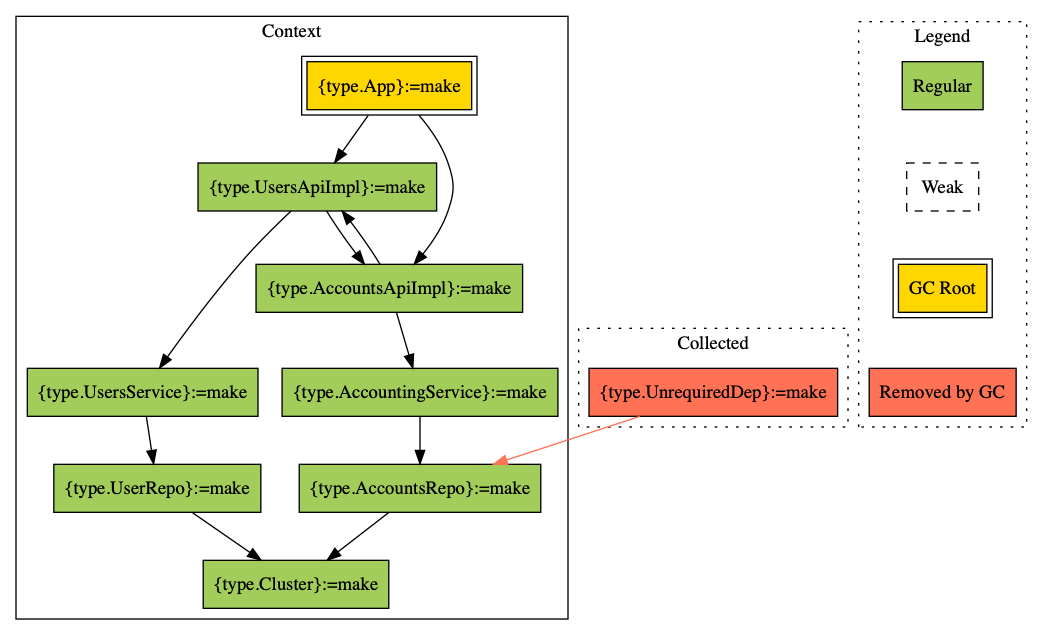
\includegraphics[width=\textwidth]{media/plan-example-dot}
  \end{figure}
  \footnotetext[1]{This picture has been generated automatically by distage extension}
\end{frame}

\begin{frame}[fragile]
\frametitle{Plan Introspection: plan dumps}
\begin{scalacode}
println(plan.render) // look for the circular dependency!
\end{scalacode}

\begin{figure}
    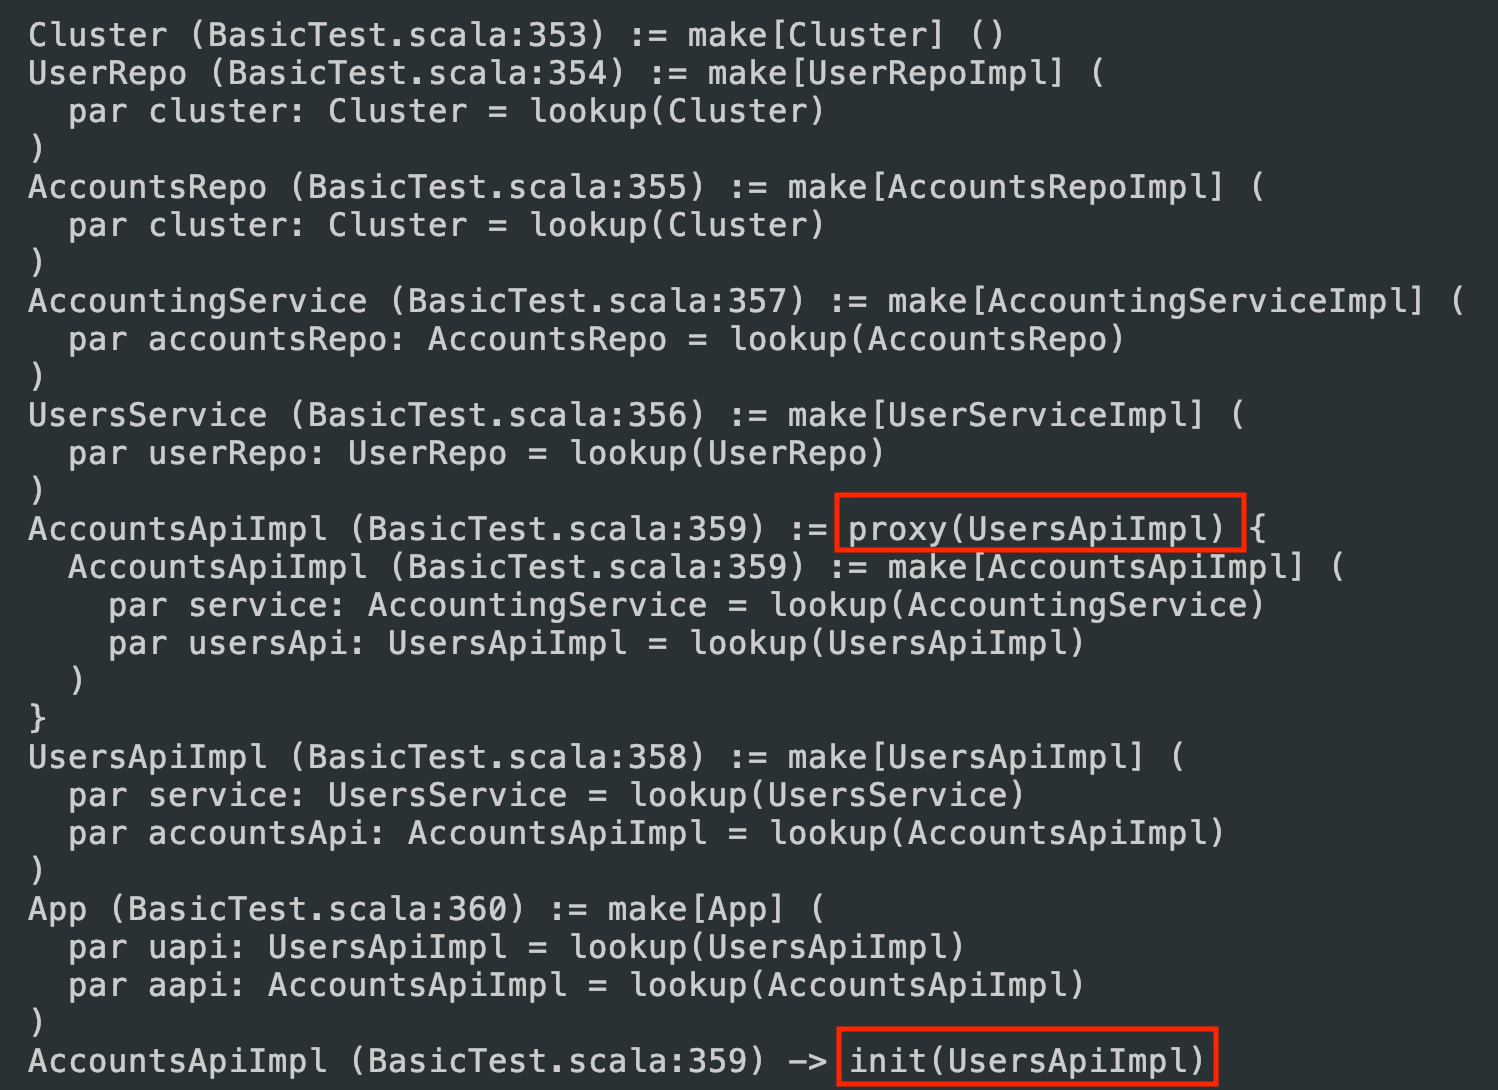
\includegraphics[width=0.75\textwidth]{media/plan-example.png}
\end{figure}
\end{frame}

\begin{frame}[fragile]
\frametitle{Plan Introspection: dependency trees}
You may explore dependencies of a component:

\begin{scalacode}
val dependencies = plan.topology.dependencies
println(dependencies.tree(DIKey.get[AccountsApiImpl]))
\end{scalacode}

\begin{figure}
    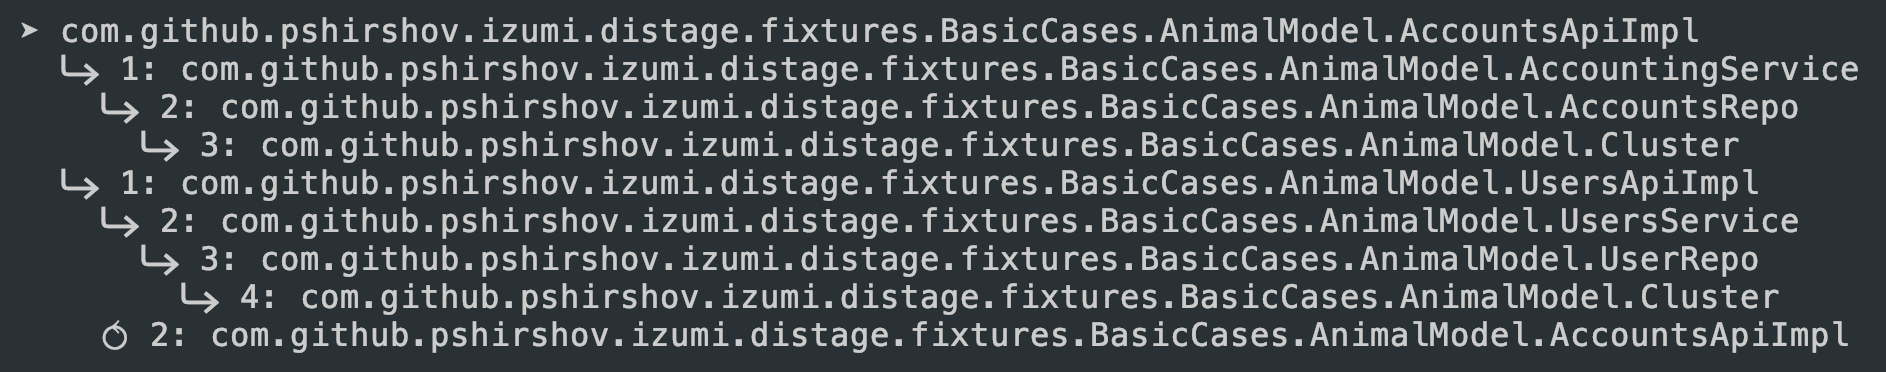
\includegraphics[width=\textwidth]{media/dependency-tree.png}
\end{figure}

Circular dependencies are specifically marked.
\end{frame}

\begin{frame}[fragile]
\begin{center}
\frametitle{Compile-Time and Runtime DI}
A Plan:
\begin{textcode}
myRepository := create[MyRepository]()
myservice    := create[MyService](myRepository)
\end{textcode}

May be interpreted as:

\begin{columns}

\begin{column}[T]{0.5\textwidth}
   \setlength{\topsep}{0pt}
   \setlength{\partopsep}{0pt}
Code tree (compile-time):
\begin{scalacode}
val myRepository =
    new MyRepository()
val myservice =
    new MyService(myRepository)
\end{scalacode}
\end{column}

\begin{column}[T]{0.5\textwidth}
Set of instances (runtime):
\begin{scalacode}
plan.foldLeft(Context.empty) {
case (ctx, op) =>
    ctx.withInstance(
        op.key
        , interpret(action)
    )
}
\end{scalacode}
\end{column}

\end{columns}
\end{center}
\end{frame}

%%%%%%%%%%%%%%%%%%%%%%%%%%%%%%%%%%%%%%%%%%%%%%%%%%%%%%%%%%%%%%%%%%%%%%%%%%%%%%%%%%%%%%%%%%%%%%%%%%%
\section{7mind stack}
\begin{frame}
  \begin{figure}
  \Huge
  \color{RubineRed} dist✪ge
  \noindent
  \rule{\linewidth}{1mm}
  \Large 7mind Stack
  \rule{\linewidth}{1mm}
  \end{figure}
\end{frame}

\begin{frame}[fragile]
  \frametitle{\distage: status and things to do}
  \distage{} is:
  \begin{enumerate}
    \item ready to use,
    \item in real production,
    \item all Run-time features are available,
    \item all Compile-time features except of full Producer are available.
  \end{enumerate}
  \vspace{0.3cm}
  Our plans:
  \begin{enumerate}
    \item \code{ProducerF\lbrack\_\rbrack} --- Producer within a monad,
    \item New Roles API,
    \item Scala.js support,
    \item Compile-time Producer,
    \item Isolated Classloaders for Roles (in future),
    \item Check our GitHub: https://github.com/pshirshov/izumi-r2.
  \end{enumerate}
\end{frame}

\begin{frame}
  \frametitle{\distage is just a part of our stack}
  We have a vision backed by our tools:
  \begin{enumerate}
    \item Idealingua: transport and codec agnostic gRPC alternative with rich modeling language,
    \item LogStage: zero-cost logging framework,
    \item \textit{Fusional Programming and Design} guidelines. We love both FP and OOP,
    \item \textit{Continous Delivery} guidelines for Role-based process,
    \item \textit{Percept-Plan-Execute} Generative Programming approach, abstract machine and computational model.
    Addresses Project Planning (see Operations Research). Examples: orchestration, build systems.
        %  Roles: distributed development without distributed computing
  \end{enumerate}

  Altogether these things already allowed us to significantly reduce development costs and
  delivery time for our client.\newline

  More slides to follow.
\end{frame}

\begin{frame}
  \begin{center}
  \Huge
  You use \texttt{Guice}?

  Switch to \distage!

  \begin{figure}
      
\includegraphics[width=0.35\textwidth]{media/haruhi.jpg}
  \end{figure}

  \end{center}
\end{frame}

\begin{frame}[fragile]
  \frametitle{Teaser: LogStage}
  A log call \dots
  \begin{scalacode}
log.info(s"$user logged in with $sessionId!")
  \end{scalacode}

  \dots may be rendered as a text like \texttt{17:05:18 UserService.login user=John Doe logged in with sessionId=DEADBEEF!}

  \dots or a structured JSON:
  \begin{jsoncode}
{
  "user": "John Doe",
  "sessionId": "DEADBEEF",
  "_template": "$user logged in with $sessionId!",
  "_location": "UserService.scala:265",
  "_context": "UserService.login",
}
  \end{jsoncode}
\end{frame}

\begin{frame}[fragile]
  \frametitle{Teaser: Idealingua}
  \begin{textcode}
id UserId { uid: str }
data User {  name: str /* ... more fields */ }
data PublicUser {
 + InternalUser
 - SecurityAttributes
}
adt Failure = NotFound | UnknownFailure
service Service {
  def getUser(id: UserId): User !! Failure
}
  \end{textcode}

\begin{enumerate}
\item Convenient Data and Interface Definition Language,
\item Extensible, transport-agnostic, abstracted from wire format,
% \item Server-to-Server, Server-to-Client \& Client-to-Server communication,
% \item Bifunctor Error Model, Strongly typed API calls - no longer remove type safety with microservices!
% \item <IMG>twitter microservices are a great way to remove typesafety</IMG>
\item JSON + HTTP / WebSocket at the moment,
\item C\#, go, Scala, TypeScript at the moment,
\item Better than gRPC / REST / Swagger/ etc.
\end{enumerate}
\end{frame}

\begin{frame}
    \frametitle{Thank you for your attention}

    \begin{center}
      distage website: https://izumi.7mind.io/

      We're looking for clients, contributors, adopters and colleagues ;)
    \end{center}

    About the author:
    \begin{enumerate}
        \item coding for 18 years, 10 years of hands-on commercial engineering experience,
        \item has been leading a cluster orchestration team in Yandex, ``the Russian Google'',
        \item implemented ``\textit{Interstellar Spaceship}'' -- an orchestration solution to manage 50K+ physical machines across 6 datacenters,
        \item Owns an Irish R\&D company, https://7mind.io,
        \item Contact: team@7mind.io,
        \item Github: https://github.com/pshirshov
        \item Download slides: https://github.com/7mind/slides/
    \end{enumerate}
\end{frame}

\begin{frame}
    \frametitle{Thank you for your attention}

    \begin{center}
      distage website: https://izumi.7mind.io/

      We're looking for clients, contributors, adopters and colleagues ;)
    \end{center}

    About the author:
    \begin{enumerate}
        \item coding for 18 years, 10 years of hands-on commercial engineering experience,
        \item has been leading a cluster orchestration team in Yandex, ``the Russian Google'',
        \item implemented ``\textit{Interstellar Spaceship}'' --- an orchestration solution to manage 50K+ physical machines across 6 datacenters,
        \item Owns an Irish R\&D company, https://7mind.io,
        \item Contact: team@7mind.io,
        \item Github: https://github.com/pshirshov
        \item Download slides: https://github.com/7mind/slides/
    \end{enumerate}
\end{frame}

\end{document}
